\chapter{Dynamics Without Solar Perturbations}
\label{chap:dynamics_without_solar_perturbations}
\graphicspath{{Results/}}

In this chapter, we will analyze the orbital motion of regolith in presence of a non-uniform gravity field, i.e. the \gls{CDE} gravity model, but in the absence of all Solar perturbations. We try to understand the general behavior of regolith under such circumstances first so that we can later understand the effect of adding Solar perturbations.

\section{Simulation Setup}
\label{sec:simulation_setup_noSP}
Since the aim is to understand the general characteristic behavior of regolith orbiting an elongated asteroid with a non-uniform gravity field, we chose the launch site to be on the longest edge of the asteroid, i.e. longitude and latitude both \SI{0}{\degree}. This launch site was chosen because it offers an easy and intuitive demarcation of particles being launched in or against the direction of asteroid's rotation. This demarcation is non-intuitive for any other general launch site, such as the one on the leading edge of the asteroid.
%
\newline\newline
%
Multiple particles are launched from the surface, forming the shape of a cone. The launch declination angle was fixed to be a general value of \SI{45}{\degree} and the launch azimuth angle was varied from 0 to \SI{359}{\degree}, thereby launching regolith in every possible direction for a given declination value. The launch velocity was varied from 1 to \SI{16}{\metre \per \second}. Thus, in total 5760 particles were launched and simulated, each with unique initial conditions.

\section{Final Fate Characteristics}
\label{sec:final_fate_characteristics_noSP}
This section will discuss the final fates encountered, when several particles are lofted from the surface of an ellipsoidal asteroid, and relate them with the initial conditions.
% The results presented in this section are a direct consequence of an attempt to understand any link between how a particle was launched and what their final outcome is. This, of course, was done in the absence of any external disturbance apart from the non-uniform gravity field so as to reduce the number of contributing factors for uncertainty. The initial intention of performing this part of the research was to discover the said link(s) through investigative methods and then later exploit it for space exploration activities.

\subsection{General Behavior}
\label{subsec:general_behavior_noSP}
\Cref{fig:final_fate_hist_noSP} depicts the final fates acquired by particles for each of the launch velocities (expressed in the \gls{ARF}). At the extreme ends of the launch velocity range, we can see that the final fate is absolute. If the launch velocity is extremely small then all particles just re-impact the surface and if the velocity is very large, then the particles simply escape. For all other launch velocities in between, the distribution of final fates is mixed, with re-impact gaining more prominence over escape if the velocity is relatively lower and vice-versa.
%
\newline\newline
%
We compare the final fate behavior in \Cref{fig:final_fate_hist_noSP} for an ellipsoidal asteroid, with the escape behavior for a spherical asteroid shown in \Cref{fig:conservative_spherical_asteroid_escape}. For the former, it is observed that escape situations occur for launch velocities as low as \SI{4}{\metre\per\second} while for the latter, they start occurring only at \SI{11}{\metre\per\second}. The complete re-impact/escape histogram for the spherical asteroid is shown in \Cref{fig:spherical_asteroid_10km_histogram}. Clearly, the number of escape cases for the ellipsoidal asteroid is much higher than that for the spherical asteroid. There are two reasons for this, first being the relatively higher inertial speed of the particle at rest for the given launch site on the ellipsoidal asteroid, i.e. \SI{6.623}{\metre\per\second}, compared to just \SI{3.312}{\metre\per\second} for the spherical asteroid. The difference is because the longest axis of the ellipsoidal asteroid, from where the particles were lofted, is \SI{20}{\kilo\metre}; whereas in case of the spherical asteroid, the particles were launched from an equatorial location and the radius of the sphere was \SI{10}{\kilo\metre}. The second reason for the lower number of escaped particles in case of the spherical asteroid is its relatively higher gravity potential value at the launch site, i.e. \SI{89.4403}{\metre\squared\per\second\squared}, compared to \SI{58.155}{\metre\squared\per\second\squared} for the ellipsoidal asteroid.
%
\newline\newline
%
If we launch particles from an equatorial site on a spherical asteroid of radius \SI{20}{\kilo\metre} for the same launch conditions as the ellipsoidal asteroid case, then the inertial speed of the particle at rest is the same for both asteroids but the gravity potential is \SI{357.761}{\metre\squared\per\second\squared} at the launch site. In such a situation, all particles re-impacted and there were no escape cases since the guaranteed escape speed was much higher and all launch velocities (1 to \SI{16}{\metre\per\second}) were below it. The variation in the \gls{CGES} curve with launch azimuth, for the spherical asteroid of radius \SI{20}{\kilo\metre}, is shown in \Cref{fig:spherical_asteroid_20km_conservative_escape_speed}.
%%%
\begin{figure}[htb]
\centering
\captionsetup{justification=centering}
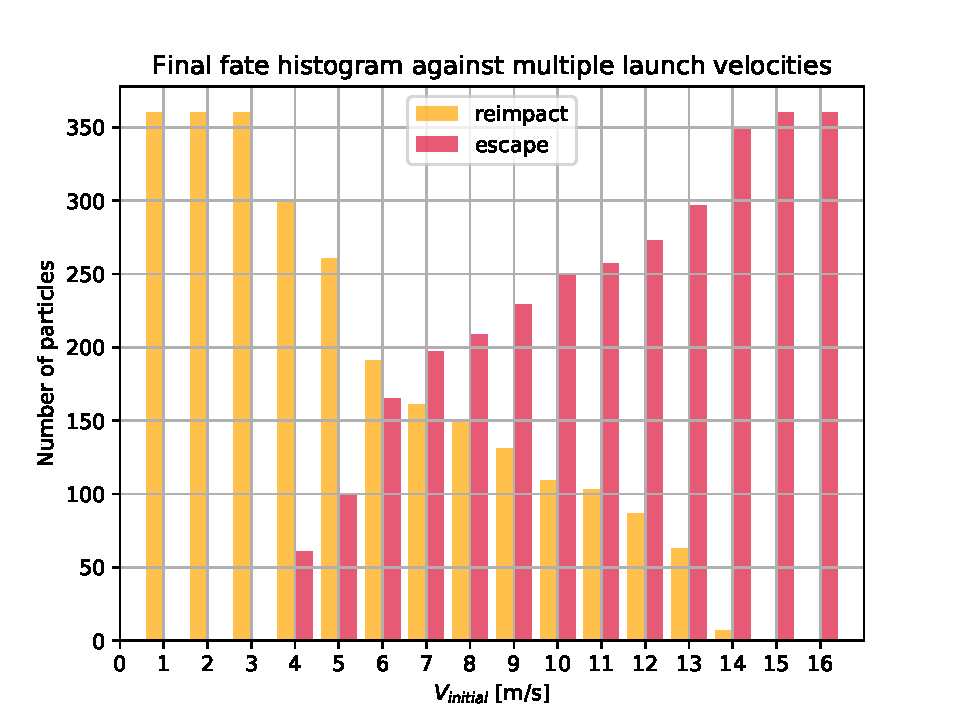
\includegraphics[width=\textwidth, height=0.4\textheight, keepaspectratio=true]{Images/longest_edge_no_perturbations/final_fate_histogram_all_velocities.pdf}
\caption{Re-impact/escape outcomes against launch velocities, which are expressed in the \gls{ARF}. The values on the y-axis represent the number of particles that acquired each of the distinct final fates for every launch velocity and are not to be confused with the launch azimuth values.}
\label{fig:final_fate_hist_noSP}
\end{figure}
\FloatBarrier
%%%
An important thing to notice is the lack of particles with temporary capture as their final fate in \Cref{fig:final_fate_hist_noSP}. Recall from \Cref{sec:assumptions} that each particle or regolith is simulated for a maximum of 270 days. So upon closer examination of the output databases, it was found that their are a few particles which did not re-impact nor escape at the end of the 270 days simulation. These particles were not temporarily captured by the asteroid, but instead, each particle was found to be on a single orbit with extremely large semi-major axis and eccentricity. Soon after launch, these particles went extremely far away from the asteroid and never returned back in the vicinity of the asteroid within the total time set for the simulation. These are not capture orbits since the definition requires them to perform multiple orbital revolutions around the asteroid for hundreds of days. Moreover, these are the particles that eventually get whisked away from the asteroid's gravity pull because of Solar perturbations (observed when simulations were run with \gls{SRP} and \gls{STBE}).
%%%
\begin{figure}[htb]
\centering
\captionsetup{justification=centering}
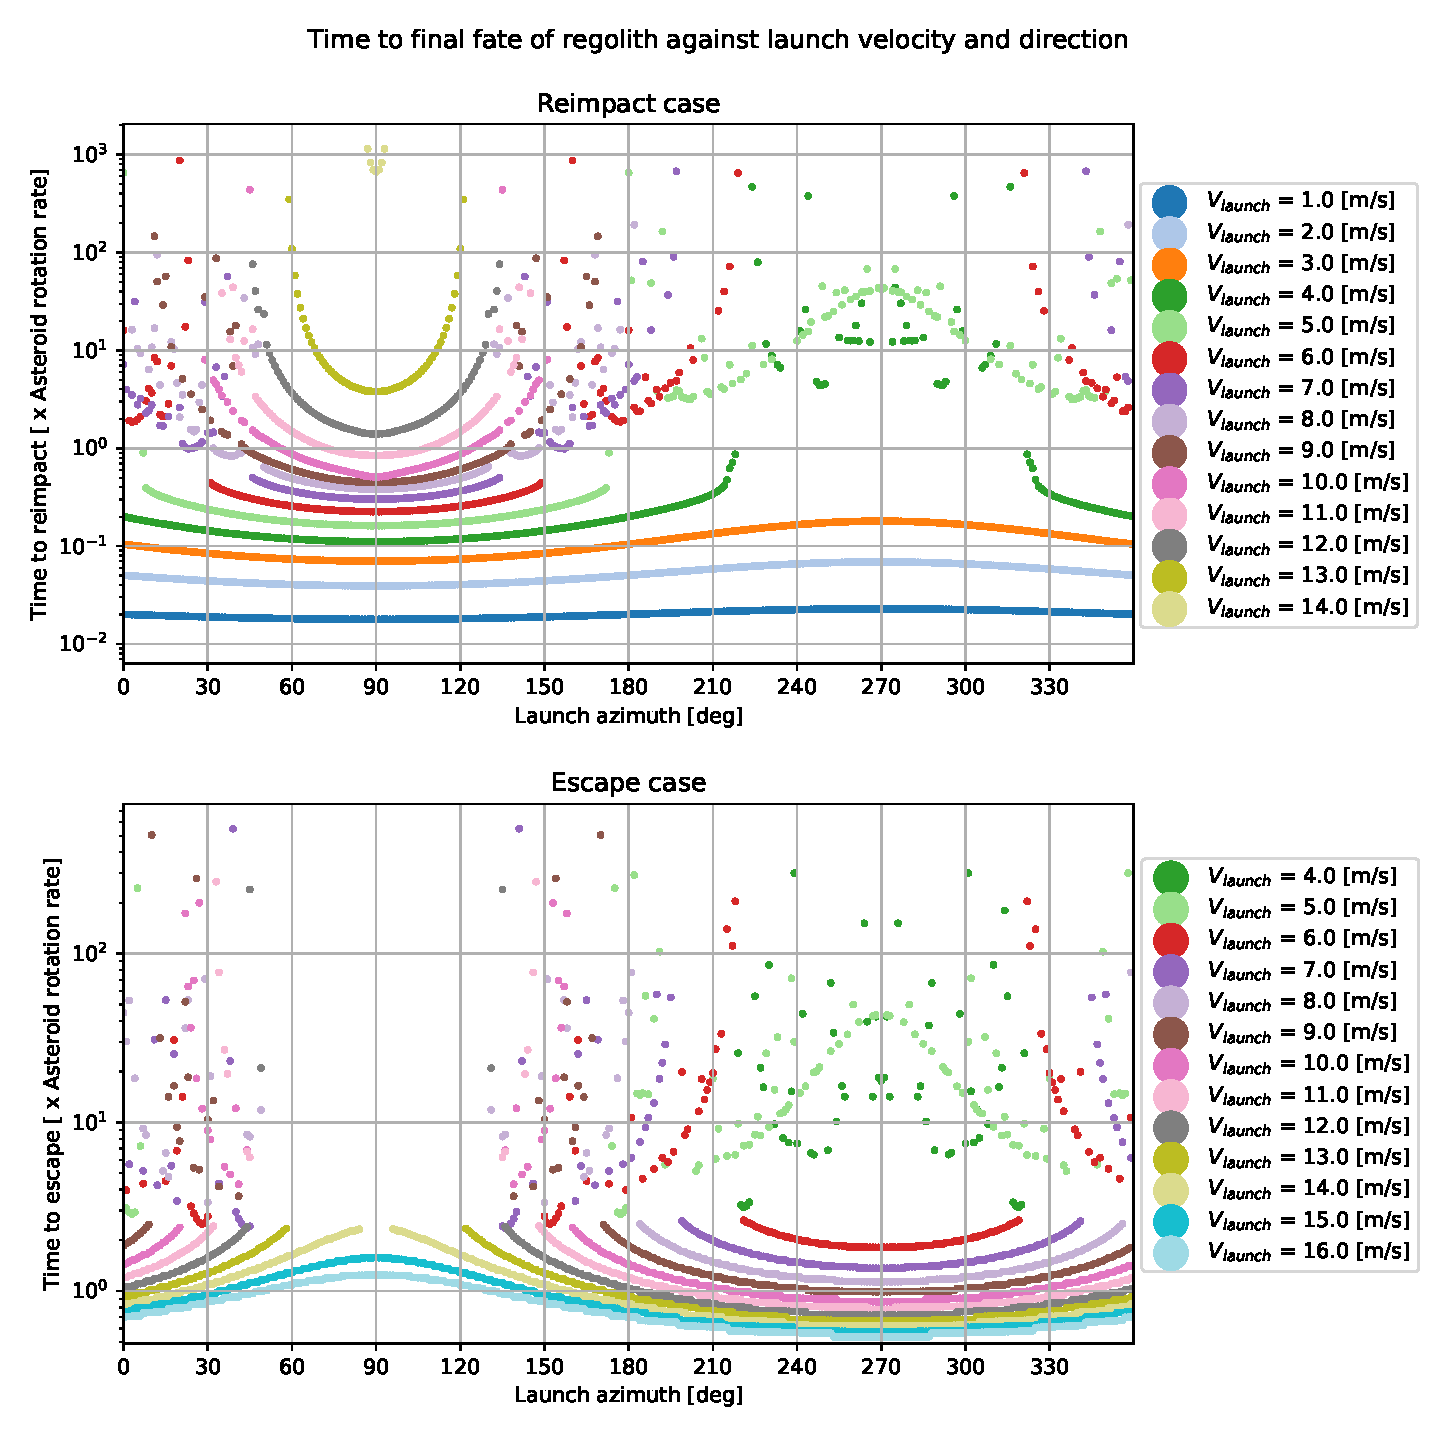
\includegraphics[width=\textwidth, height=\textheight, keepaspectratio=true]{Images/longest_edge_no_perturbations/time_to_final_fate_all_velocities_newLegend.pdf}
\caption{Total time taken by regolith to meet their respective final outcomes, as a function of launch azimuth and launch velocity. The time values are mentioned as a multiple of the asteroid rotation rate which is 5.27 hours.}
\label{fig:final_fate_time_noSP}
\end{figure}
\FloatBarrier
%%%
\Cref{fig:final_fate_time_noSP} shows the total time taken by regolith, launched with different launch conditions, to meet their respective final fates. The plot shows that, for the same final fate, its not not just the launch velocity but the direction of launch as well that can have a significant impact on the total time it takes to meet a given fate. For a given launch velocity and say the escape case, we can see that if the particle is launched in the direction of the rotation (for example, azimuth = \SI{270}{\degree}), then it gets an extra boost from the asteroid's rotation and results in taking lesser time to escape. This is relative to being launched in a direction opposite to the asteroid's rotation (for example, azimuth = \SI{90}{\degree}), where the particle's inertial velocity reduces and hence takes more time to escape. This situation with launch direction and time to final fate gets reversed when we consider the case of re-impact. Thus for the same velocity, when launched in the direction of asteroid's rotation, the particle tends to go further away from the asteroid because of an excess velocity provided by the rotation which then results in more time for the particle to come back and re-impact the surface.
%
\newline\newline
%
The directional behavior for escape or re-impact is not always as smooth as we just discussed. This is observed in the chaotic distribution of few of the data points in \Cref{fig:final_fate_time_noSP}. Note that these observations are also only for those cases where a launch velocity results in both escape and re-impact situations. For example, if we look at the case of \SI{4}{\metre\per\second} in \Cref{fig:final_fate_time_noSP}, we observe that the time to escape for launch azimuth \SI{270}{\degree} is lower than that for a few launch azimuths below \SI{270}{\degree}. This happens because of a complex interaction between the orbiting particle and a rapidly rotating asteroid with non-uniform gravity field. We now look at the velocity extremes in \Cref{fig:final_fate_hist_noSP} which result either only in a re-impact or escape, and observe their orbital time in \Cref{fig:final_fate_time_noSP}. It is observed that the time to achieve the respective final fates is extremely small and mostly in fractions of the asteroid's rotation rate. This means that these particles do not spend enough time in orbit to get affected by the non-uniform gravity field or the asteroid's rotation and hence show no exceptional behavior as discussed before.
% The most notable example for this is the escape scenarios for the launch velocity of \SI{4}{\metre \per \second}. For the current example, escape occurs only when the launch azimuth is favorable, i.e. when the particles are launched in the rotational direction, in addition to a complex interaction with the fast rotating asteroid and irregular gravity field. So for the example of \SI{4}{\metre \per \second}, escape occurs not because the velocity is inherently high enough but because of the interaction with the asteroid, which is why a chaotic behavior for it is observed in \Cref{fig:final_fate_time_noSP}.

\subsection{Re-impact behavior}
This section will discuss certain characteristic behavior that is specific to the re-impact scenario. \Cref{fig:crashmap_all_noSP} shows a map of re-impact locations on the surface of the asteroid for all launch velocities that led to this particular fate. The distinction due to launch azimuth is not plotted explicitly. The qualitative map in the plot is simply a 2D histogram plot with hexagonal shaped bins. These bins do not represent the number of particles within a given location but instead represent the range of initial launch velocities that led to re-impact in that location. From the qualitative map, we can observe that particles launched with the lowermost velocities mostly re-impact very close to the launch site itself. The intermediate velocities seem to confine the re-impact locations within the \SI{-30}{\degree} to \SI{+30}{\degree} latitude range and lie mostly on the West of the launch site. And finally, the higher velocity range confine the particles to re-impact mostly along the uppermost and lowermost latitudes.
%
\newline\newline
%
Thus the qualitative map gives an excellent description of how the re-impact locations change with increasing launch velocities. The map with the actual re-impact locations in \Cref{fig:crashmap_all_noSP} shows that the bulk of all re-impacted particles lie around the two longest edges of the asteroid. Everywhere in between has a very scarce distribution of particles. A pattern in the re-impact location becomes apparent if one visualizes the launch azimuth angles, especially for the lower launch velocity range and is discussed shortly.
%%%
\begin{figure}[htb]
\centering
\captionsetup{justification=centering}
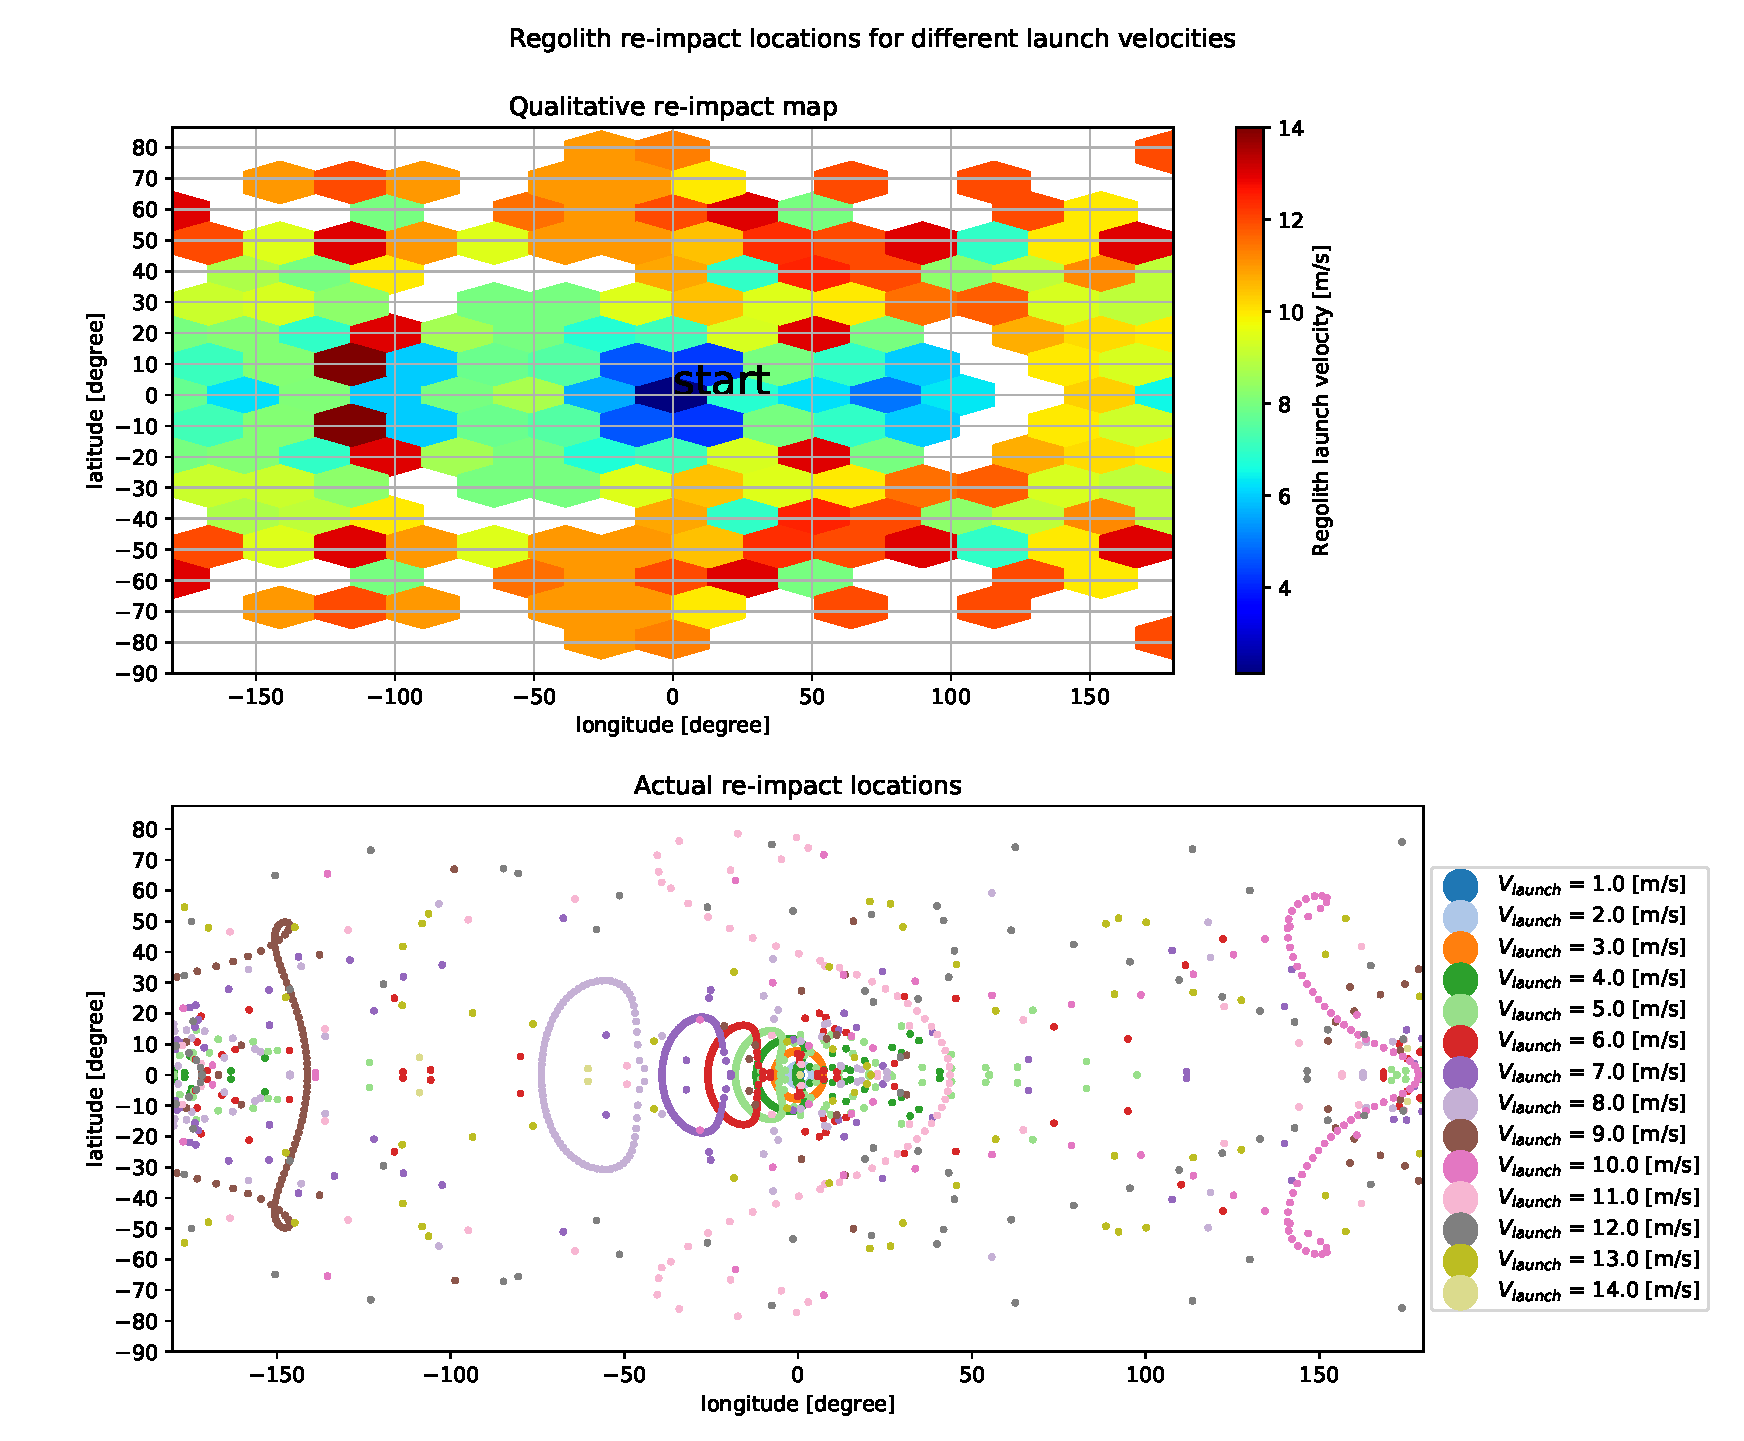
\includegraphics[angle=90, width=\textwidth, height=\textheight, keepaspectratio=true]{Images/longest_edge_no_perturbations/crash_map_all_velocities_noGrid.pdf}
\caption{Regolith re-impact locations marked for all launch velocities that eventually lead to it. A qualitative map is shown as well that provides a general idea on re-impact locations and is color coded based on the regolith launch velocity.}
\label{fig:crashmap_all_noSP}
\end{figure}
\FloatBarrier
%%%
We look a bit more in detail into the re-impact location map for three different velocities. These velocities are chosen such that, by studying them, we can estimate the behavior for the low, intermediate and high launch velocities. In addition to this, we also look at the effect of the launch direction on re-impact location and see if there is a link between them or if it is all chaotic.
%%%
\begin{figure}[htb]
\centering
\captionsetup{justification=centering}
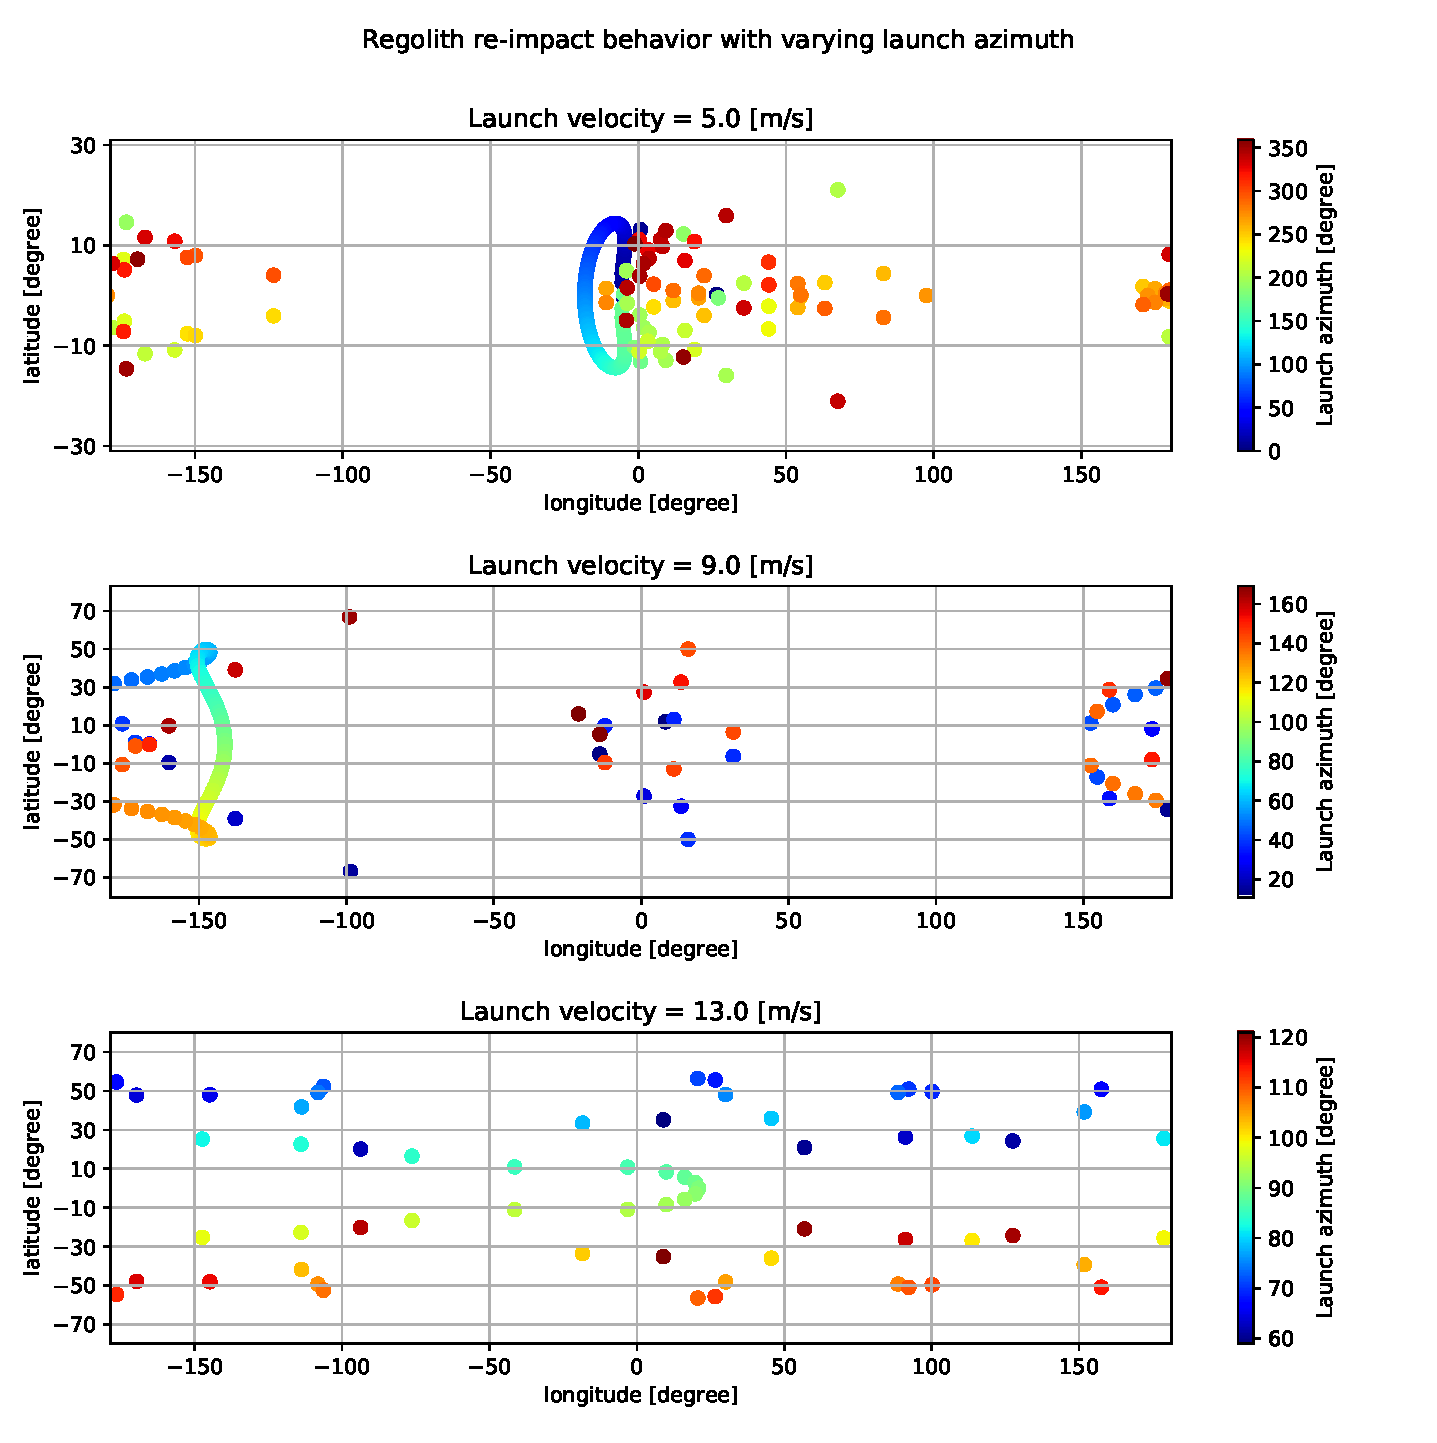
\includegraphics[width=\textwidth, height=0.6\textheight, keepaspectratio=true]{Images/longest_edge_no_perturbations/re-impact_behavior_with_azimuth.pdf}
\caption{Single velocity re-impact location maps for three different velocities. The re-impact locations are color coded based on the launch azimuth.}
\label{fig:crashmap_launchAzimuth_noSP}
\end{figure}
\FloatBarrier
%%%
For the launch velocity of \SI{5}{\metre \per \second}, the re-impact locations corresponding to launch azimuth angles that are against the asteroid's rotational direction (more specifically \SI{7}{\degree} to \SI{173}{\degree})\footnote{Trajectories for launch azimuths \SI{1}{\degree} to \SI{6}{\degree} and \SI{174}{\degree} to \SI{179}{\degree} get assisted by the fast rotating asteroid which results in them entering escape trajectories}, form a distinct curve West of the launch location. These are the particles that soon after launch, re-impact the surface without completing even a single orbit because their energy is reduced significantly enough by the opposing direction of the gravity field. And since the initial launch velocity was inherently small, these particles are not able to reach far away from the launch site either. Launch azimuths \SI{0}{\degree} and \SI{180}{\degree} are not directly against or into the asteroid's rotational direction and the corresponding particles complete multiple revolutions before re-impacting the asteroid's surface. Their re-impact location is \SI{0.2}{\degree} latitude and \SI{26.6}{\degree} longitude and can be seen in \Cref{fig:crashmap_launchAzimuth_noSP}. The remaining launch azimuth angles, i.e. the ones that launch the particle in the asteroid's rotational direction \footnote{Not all of these result in re-impact, a few of these also result in an escape scenario but that is irrelevant for the discussion at hand}, results in a more oddly distributed re-impact locations. The asteroid's rotation assists the launch such that the particles complete one or more orbital revolutions (observed from individual trajectory plots) before re-impacting the surface. This is why for these azimuth angles, the re-impacted particles are not evenly distributed in a smooth curve on the East side of the launch site as the trajectories are not simply ballistic. The re-impact locations in 3D for this launch velocity are shown in \Cref{fig:crashmap_3d_5ms_noSP}.
%%%
\begin{figure}[htb]
\centering
\captionsetup{justification=centering}
\subfloat[]{
    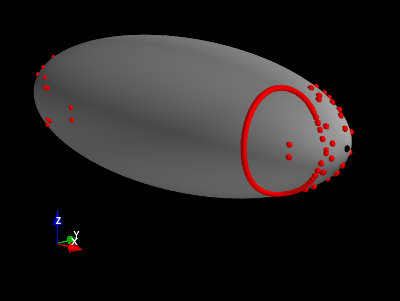
\includegraphics[width=0.5\textwidth, height=0.5\textheight, keepaspectratio=true]{Images/longest_edge_no_perturbations/5ms_crashMap_view1.png}
    \label{fig:crash_3d_5ms_view1}
}
\subfloat[]{
    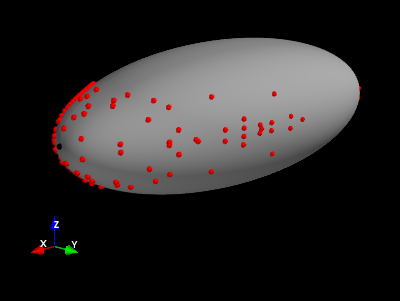
\includegraphics[width=0.5\textwidth, height=0.5\textheight, keepaspectratio=true]{Images/longest_edge_no_perturbations/5ms_crashMap_view2.png}
    \label{fig:crash_3d_5ms_view2}
}

\subfloat[]{
    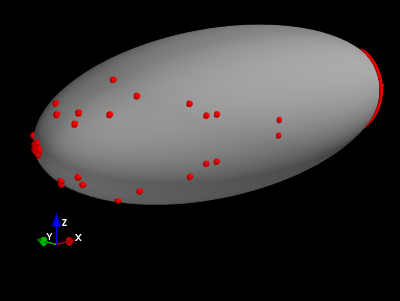
\includegraphics[width=0.5\textwidth, height=0.5\textheight, keepaspectratio=true]{Images/longest_edge_no_perturbations/5ms_crashMap_view3.png}
    \label{fig:crash_3d_5ms_view3}
}
\subfloat[]{
    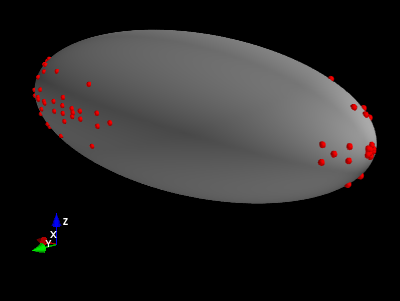
\includegraphics[width=0.5\textwidth, height=0.5\textheight, keepaspectratio=true]{Images/longest_edge_no_perturbations/5ms_crashMap_view4.png}
    \label{fig:crash_3d_5ms_view4}
}
\caption{3D view, from four different angles, of regolith re-impact locations for particles launched with a velocity of \SI{5}{\metre \per \second}. The red points represent the re-impact sites and the singular black dot represents the launch site.}
\label{fig:crashmap_3d_5ms_noSP}
\end{figure}
\FloatBarrier
%%%
Consider the re-impact locations in \Cref{fig:crashmap_launchAzimuth_noSP} for the launch velocity of \SI{9}{\metre\per\second}. Note that, for this velocity, the launch azimuth angles that result in a re-impact are only the ones which launch the particle in a direction opposite to that of the asteroid's rotation \footnote{Not all the angles within this range correspond to a re-impact situation and some result in an escape as well but the latter is not relevant to the discussion at hand}. Within this range of azimuth angles, the lowermost and the uppermost angles comprise of trajectories that are either ballistic or comprise of one or more orbital revolutions. In case of the ballistic trajectories, we do not see the behavior as we saw for the launch velocity case of \SI{5}{\metre\per\second} where the particles neatly lined up on the West side of the launch site. For the current case, the launch velocity magnitude is inherently high. We observed a particle which took the least amount of time to re-impact and also had a ballistic trajectory, and found that the asteroid had rotated a little more than \SI{315}{\degree} when the particle re-impacted the surface but on the far East end of the asteroid. Since the launch velocity is inherently high, the particle was able to achieve a high enough altitude during which the asteroid had achieved a significant amount of rotation on its own axis, which led to the aforementioned situation.
%
\newline\newline
%
There is a very distinct collection of re-impact points (the blue-green-orange curve) on the West side of the launch point, in \Cref{fig:crashmap_launchAzimuth_noSP} for the velocity of \SI{9}{\metre\per\second} and belongs to the azimuth angles from \SI{46}{\degree} to \SI{136}{\degree}. The corresponding trajectories are all ballistic in nature and impact the surface relatively sooner after launch. Since the launch velocity is inherently high, unlike in the case of \SI{5}{\metre\per\second}, these particles are able to re-impact a bit further away from the launch site. This is clearly visible in \Cref{fig:crashmap_launchAzimuth_noSP}. For the case of \SI{9}{\metre\per\second}, the 3D view of all re-impact locations is shown in \Cref{fig:crashmap_3d_9ms_noSP}.
%
\newline\newline
%
Similarly, for the launch case of \SI{13}{\metre\per\second} in \Cref{fig:crashmap_launchAzimuth_noSP}, we first notice that the window or range of launch azimuth angles has reduced further. All particle trajectories, in this case, are ballistic in nature and we do not witness a continuous line of re-impact locations, as opposed to that in the case of 5 and \SI{9}{\metre\per\second}. When launched at \SI{13}{\metre\per\second}, the ballistic trajectories are not short lived, that re-impact the surface soon after launch \footnote{Soon after launch, here, refers to the fact that the ballistic trajectories re-impacted the surface before the asteroid could complete even a single rotation on its own axis}, which would have allowed a continuous curve on surface to be formed. Since for the current case the launch velocity has a sufficiently larger magnitude, the particles are lofted into even higher altitude trajectories, taking more time to traverse. This is the fundamental difference with the other two velocity cases, as here the asteroid performs several rotations on its axis before the particles re-impact. Thus the ballistic re-impact trajectories for launch velocity of \SI{13}{\metre\per\second} shows similar behavior as that of the multi-orbital revolution cases of 5 and \SI{9}{\metre\per\second}. The re-impact locations in 3D are shown in \Cref{fig:crashmap_3d_13ms_noSP}.
%
\newline\newline
%
Thus, for lower launch velocities, a continuous curve of re-impact locations can be linked to the launch direction which in our case is the launch azimuth angle \footnote{The launch declination angle for our simulation was kept constant}. But the same can not be said for higher launch velocities. Another intriguing observation in \Cref{fig:crashmap_launchAzimuth_noSP} is made for the launch velocity of \SI{5}{\metre\per\second}. We see that the particle launched with azimuth angle of \SI{90}{\degree} goes further away than, for example, a particle launched with an azimuth angle of \SI{10}{\degree}. This happens even though the former launch case will experience more resistance in launch since it is directly opposite to the asteroid's rotational direction. The reason for this is simple and becomes apparent if one looks at the trajectory plots shown in \Cref{fig:5ms_traj_90and10_azim_noSP}.

\subsection{Escape Behavior}
\label{subsec:escape_behavior_noSP}
We now present a brief discussion on the particles that resulted in an escape situation, and do so for the same launch velocities used for explaining the re-impact scenarios. For these launch velocities, \Cref{fig:hev_escapeHist_noSP} shows the \gls{HEV} for all escaped regolith. As the velocity increases from 5 to \SI{13}{\metre\per\second}, we see that the distribution of particles, based on their \gls{HEV}, becomes less and less random and more streamlined. There is a link between how the particles are distributed with \gls{HEV} and the way they escape. To understand this, we take the example of \SI{9}{\metre\per\second} and look at all escape cases from below \SI{100}{\degree} in launch azimuth. A zoomed-in version of the corresponding data points from \Cref{fig:hev_escapeHist_9ms_noSP} is shown in \Cref{fig:hev_9ms_lowerAzimuths_noSP}. In the latter, we can see that for launch azimuths from \SI{0}{\degree} to \SI{9}{\degree}, the \gls{HEV} uniformly reduces and beyond that all other data points are randomly distributed. The distinction between the two regimes becomes apparent when we look at the osculating energy and eccentricity for all these data points, as shown in \Cref{fig:energy_ecc_escape_9ms_noSP}.
%%%
\begin{figure}[htb]
\centering
\captionsetup{justification=centering}
\subfloat[]{
    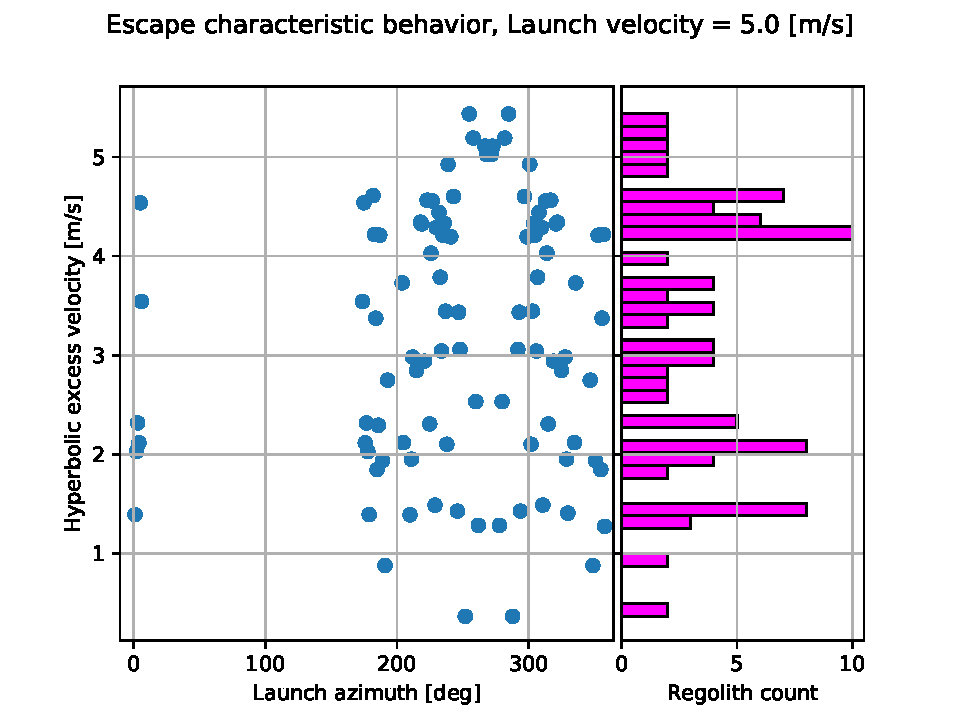
\includegraphics[width=0.5\textwidth, height=0.5\textheight, keepaspectratio=true]{Images/longest_edge_no_perturbations/escape_behavior_5ms.pdf}
    \label{fig:hev_escapeHist_5ms_noSP}
}
\subfloat[]{
    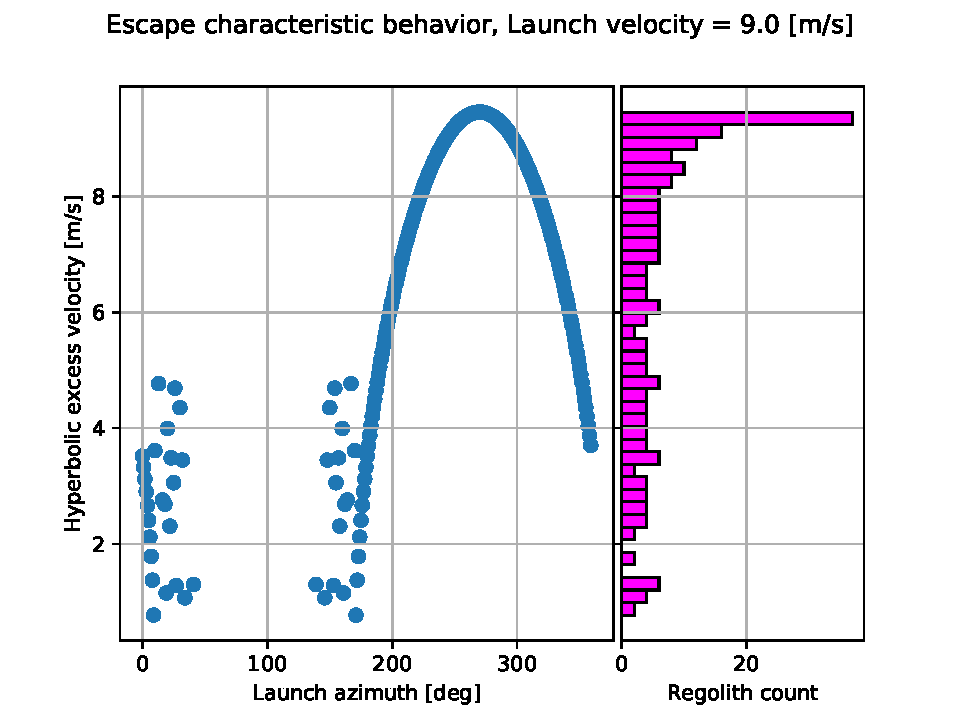
\includegraphics[width=0.5\textwidth, height=0.5\textheight, keepaspectratio=true]{Images/longest_edge_no_perturbations/escape_behavior_9ms.pdf}
    \label{fig:hev_escapeHist_9ms_noSP}
}

\subfloat[]{
    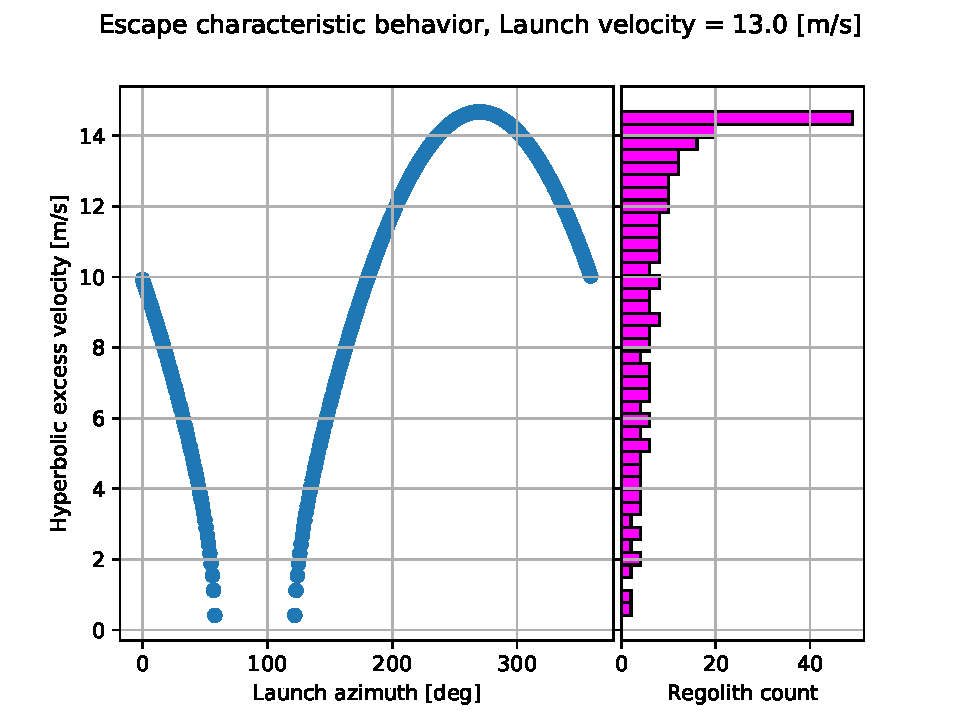
\includegraphics[width=0.5\textwidth, height=0.5\textheight, keepaspectratio=true]{Images/longest_edge_no_perturbations/escape_behavior_13ms.pdf}
    \label{fig:hev_escapeHist_13ms_noSP}
}
\caption{Hyperbolic escape velocity versus launch azimuth for three different launch velocity cases. The histogram bars in each plot depicts the number of regolith for the various hyperbolic excess velocities on the y-axis.}
\label{fig:hev_escapeHist_noSP}
\end{figure}
\FloatBarrier
%%%
So for the data points with uniformly reducing \gls{HEV} values, we observe that the energy never becomes negative and the eccentricity always stays above 1.0, which means that the corresponding regoliths are on an escape trajectory immediately after launch. It doesn't take a gravity assist from the fast rotating asteroid to put these regolith on an escape route. This is an important distinction against the randomly distributed data points in \Cref{fig:hev_9ms_lowerAzimuths_noSP}. For the latter, from the eccentricity and energy curves, we can witness that the particles briefly enter bounded orbits around the asteroid but eventually escape with a sudden increase in energy (becoming positive) and eccentricity (going above 1.0). This happens because, after launch, the particle trajectories get gravity assist from the asteroid that is sufficient to put the particle on an escape route. What was shown here for an example of \SI{9}{\metre\per\second} was not an isolated case and was found to be true for other launch velocities as well, but their results are not shown here for brevity. Also, this behavior stands true for data points with uniformly increasing \gls{HEV} values such as in the case of 9 and \SI{13}{\metre\per\second}. Thus, just by looking at the \gls{HEV} plot, we can now determine which launch azimuths led to an immediate escape and which ones required gravity assist from the asteroid to escape. The trajectory plots for a few launch azimuths that highlight this distinction is shown in \Cref{fig:escape_example_traj_9ms_noSP}.
%%%
\begin{figure}[htb]
\centering
\captionsetup{justification=centering}
\subfloat[]{
    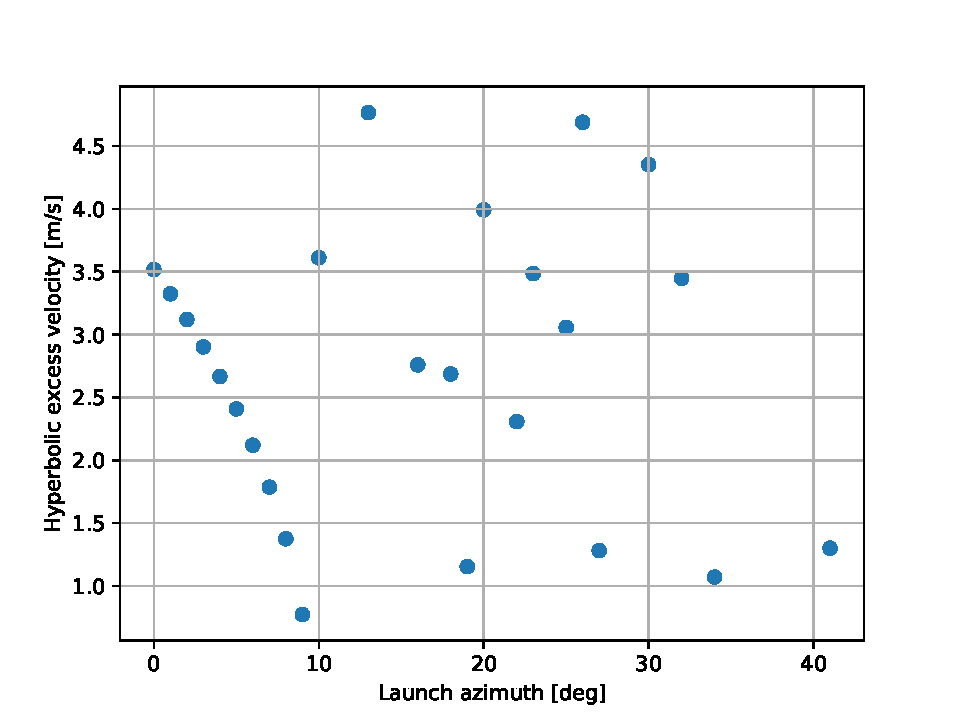
\includegraphics[width=0.5\textwidth, height=0.4\textheight, keepaspectratio=true]{Images/longest_edge_no_perturbations/escape_hev_9ms_lowerAzimuth.pdf}
    \label{fig:hev_9ms_lowerAzimuths_noSP}
}
\subfloat[]{
    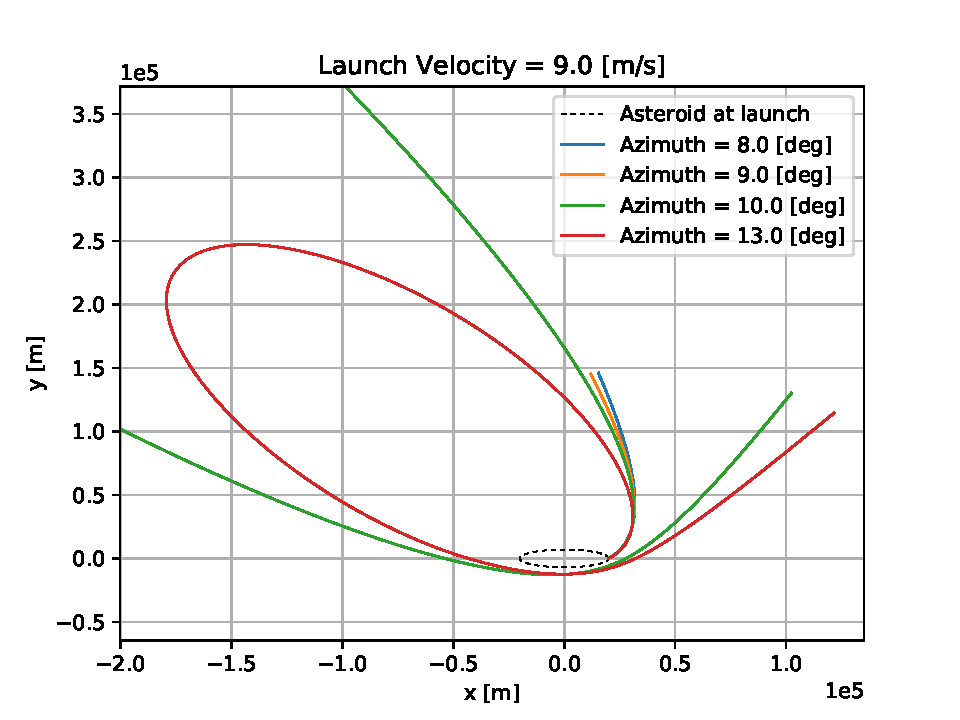
\includegraphics[width=0.5\textwidth, height=0.4\textheight, keepaspectratio=true]{Images/longest_edge_no_perturbations/9ms_escape_example_trajectories.pdf}
    \label{fig:escape_example_traj_9ms_noSP}
}
\caption{\protect\subref{fig:hev_9ms_lowerAzimuths_noSP} Zoomed-in data points for azimuth angles below \SI{100}{\degree} from \protect\Cref{fig:hev_escapeHist_9ms_noSP}. \protect\subref{fig:escape_example_traj_9ms_noSP} Example escape case trajectory plots for select few launch azimuths and a launch velocity of \SI{9}{\metre\per\second}.}
\end{figure}
\FloatBarrier
%%%
% From the previous observation, we can also confirm the pattern of variation in the \gls{HEV} values for non-chaotic data points in \Cref{fig:hev_escapeHist_noSP}. If we consider looking at the \SI{13}{\metre\per\second} case, as an example, we see that the \gls{HEV} increases with increasing launch azimuth values beyond \SI{100}{\degree} up until \SI{270}{\degree}. This happens because for increasing launch azimuths in this range, the particle's inertial launch velocity increases as well as the azimuths align more and more in the asteroid's rotational direction and becomes maximum for the exact azimuth of \SI{270}{\degree}. Now we saw earlier that these particles are inherently on an escape trajectory immediately after launch and do not require gravity assists from the rotating asteroid to be on one. This implies that if the inertial launch velocity itself is high, then the inertial velocity at the instance of escape remains high too, which is what we observe in the plots.

\subsection{Sensitivity To Launch Conditions}
\label{subsec:sensitivity_noSP}
In this section, we will briefly highlight how regolith motion is sensitive in terms of their final fate, i.e., escape or re-impact. Recalling from \Cref{sec:simulation_setup_noSP}, the launch site and launch declination angle remain constant in this simulation exercise. We vary only the launch azimuth angle and the launch velocity of the regolith while lofting them. Hence, we judge the sensitivity in terms of these two initial elements.
%
\newline\newline
%
\Cref{fig:270Azim_traj_noSP} highlights the difference between two trajectories that were launched with the same azimuth angle but differently launch velocities. An escape situation is encountered when the particle is launched with a velocity of \SI{4}{\metre\per\second} while the same particle re-impacts when launched with a velocity of \SI{5}{\metre\per\second}. With the resolution of launch conditions established in general for our simulation, and for every other launch condition being the same, the particle is sensitive to either of the final fates with \SI{1}{\metre\per\second} of a difference in the launch velocity.
%
\newline\newline
%
\Cref{fig:10ms_traj_noSP} highlights the difference between two trajectories when the launch velocity is the same, i.e. \SI{10}{\metre\per\second}, but the launch azimuths are different. So at azimuth \SI{41}{\degree}, the particle escapes while at \SI{42}{\degree} the particle re-impacts the asteroid. Thus, for all other launch conditions being the same, the particle is sensitive to either of the final fates to a \SI{1}{\degree} launch azimuth resolution.
%
\newline\newline
%
The current discussion, albeit short, was to see if the sensitivity (in terms of final fate acquired by regolith) had a magnitude equal to the resolution of varying the launch conditions in the current simulation scenario. This was found to be true, but, from all the results that we have seen so far and looking at how blurry the line is in distinguishing the two fates, a similar sensitivity behavior can be expected if the resolution of launch conditions is lowered.
%%%
\begin{figure}[htb]
\centering
\captionsetup{justification=centering}
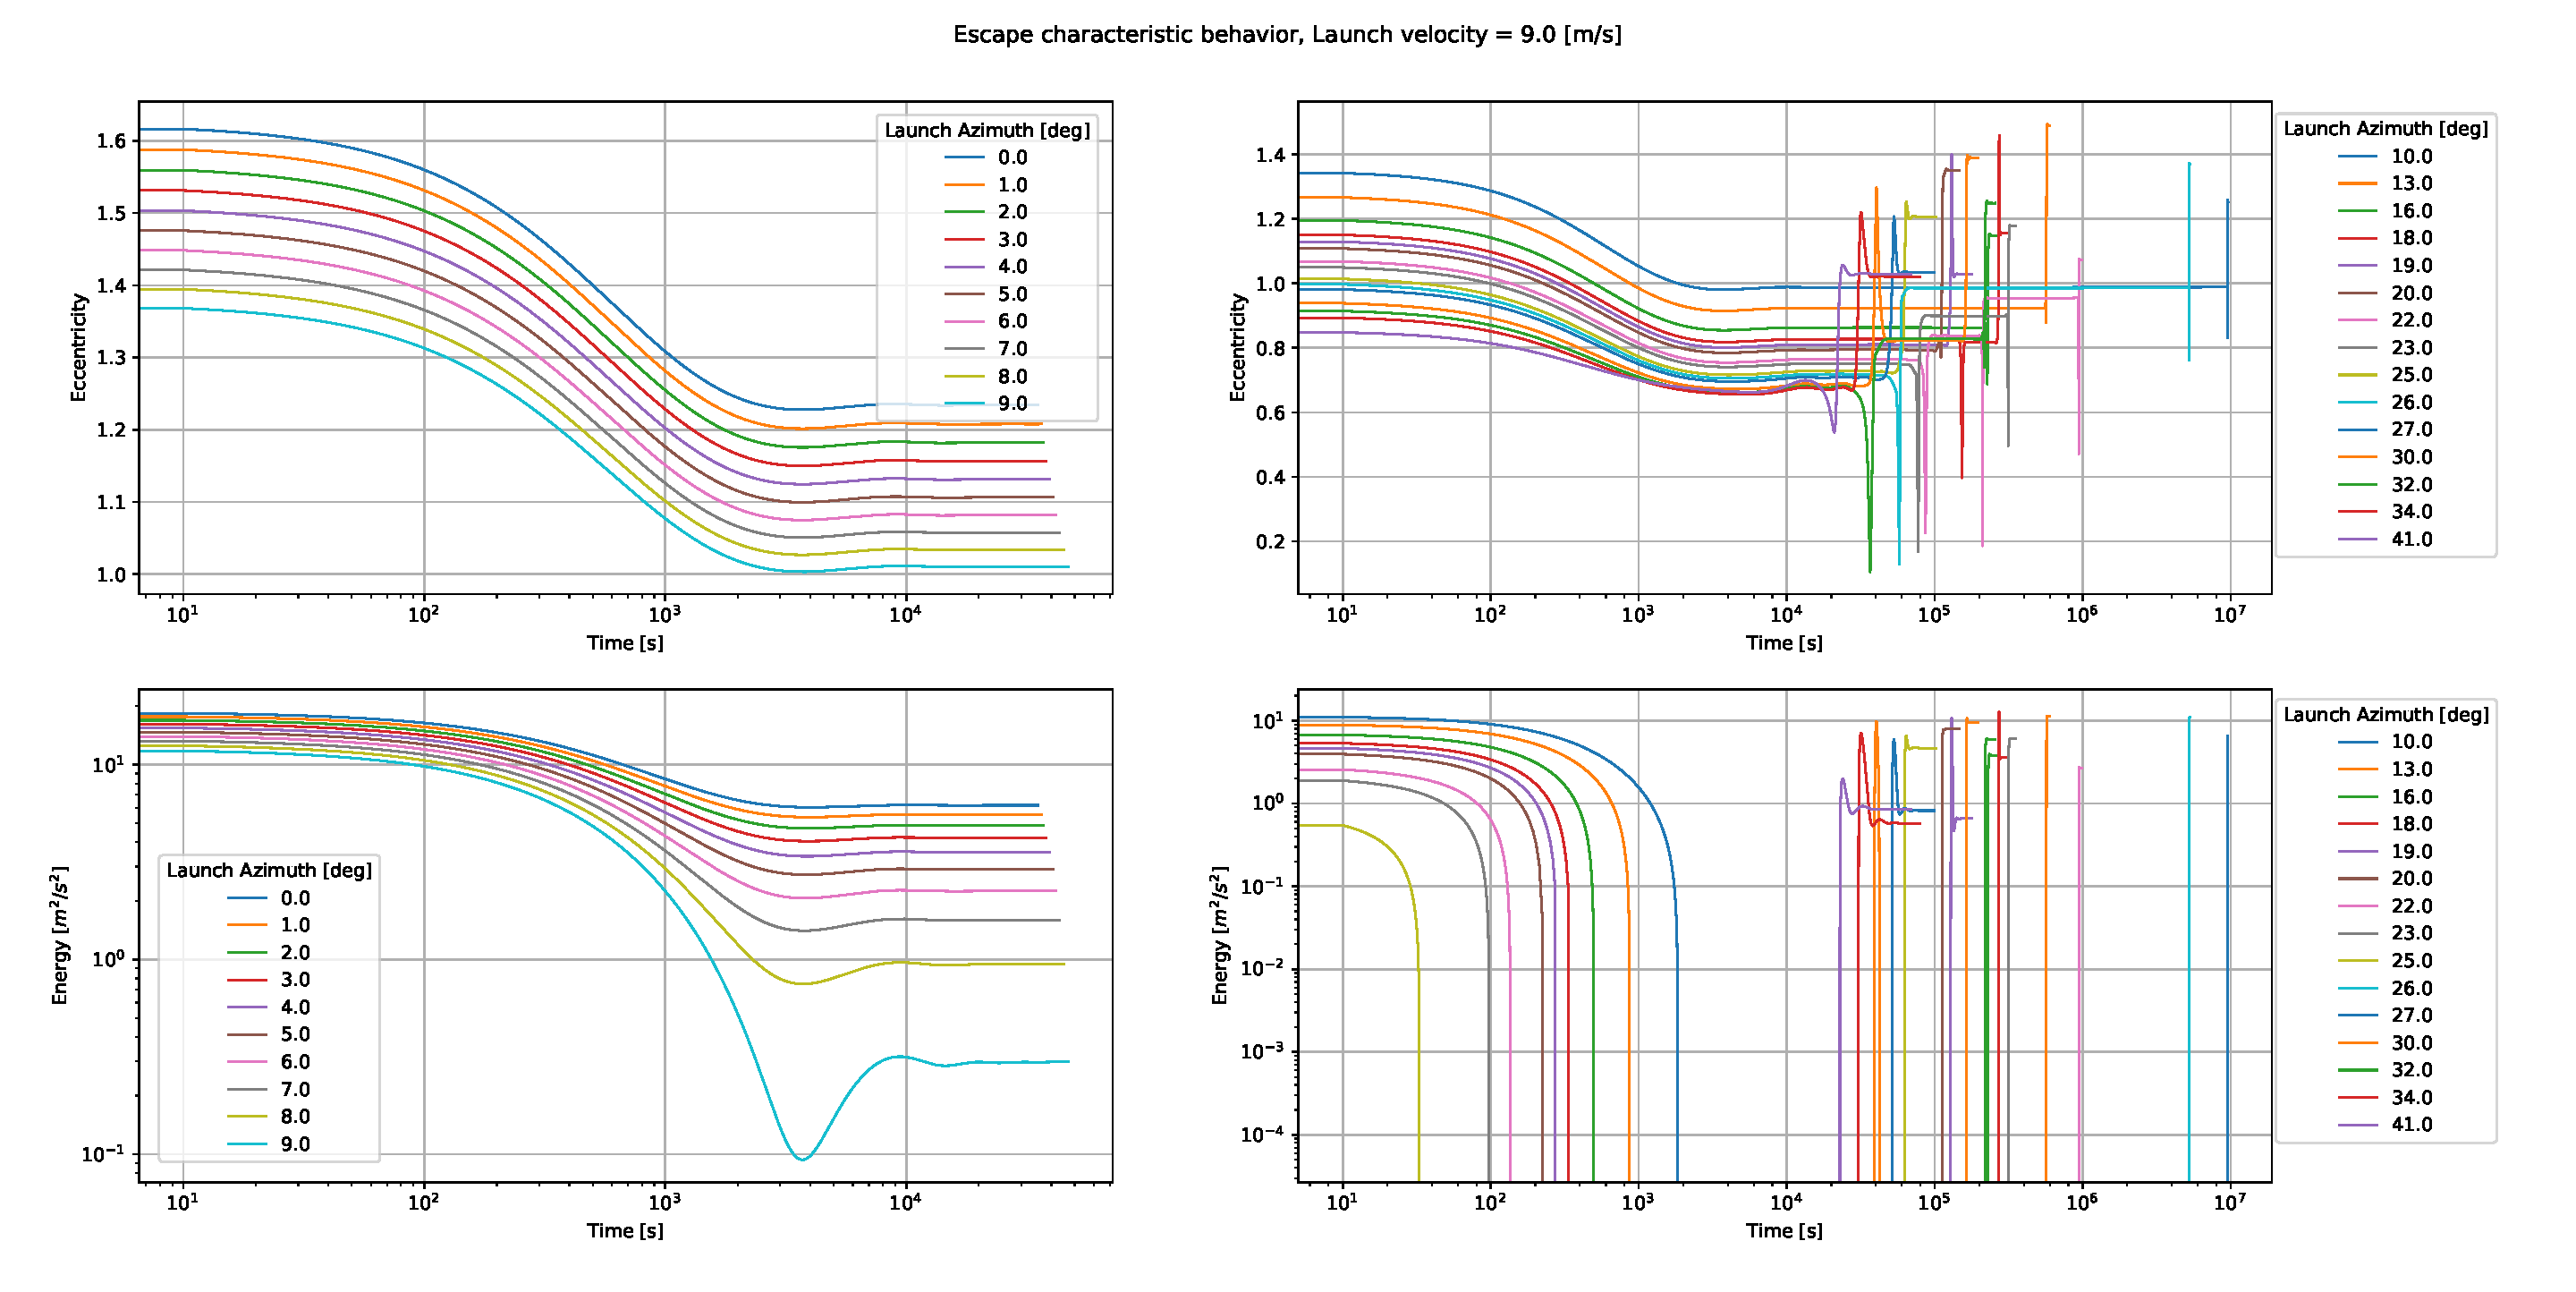
\includegraphics[angle=90, width=\textwidth, height=\textheight, keepaspectratio=true]{Images/longest_edge_no_perturbations/escape_energy_ecc_9ms.pdf}
\caption{Osculating energy and eccentricity for all escape cases as shown in \protect\Cref{fig:hev_9ms_lowerAzimuths_noSP}. The energy plot is shown in an unorthodox way by using a logarithmic scale to easily distinguish energies that stay positive for the entire duration until escape. If the energy becomes negative, then on this scale, the corresponding curve appears to be going straight downwards in the plot (since a negative value is not defined on the log scale). Similarly, if the energy becomes positive from a negative value earlier, then the curve appears to be coming upwards straight (again from some hypothetical negative value at the bottom of the log scale).}
\label{fig:energy_ecc_escape_9ms_noSP}
\end{figure}
\FloatBarrier
%%%
%%%
\begin{figure}[htb]
\centering
\captionsetup{justification=centering}
\subfloat[]{
    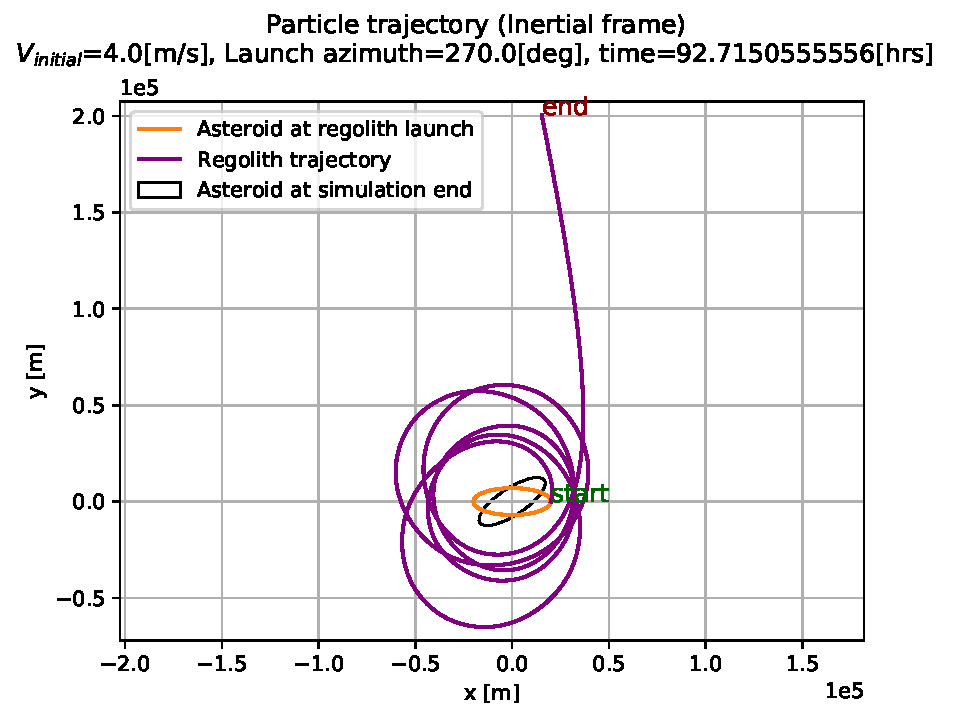
\includegraphics[width=0.5\textwidth, height=0.5\textheight, keepaspectratio=true]{Images/longest_edge_no_perturbations/4ms_270Azim_escape.pdf}
    \label{fig:4ms_270Azim_traj_noSP}
}
\subfloat[]{
    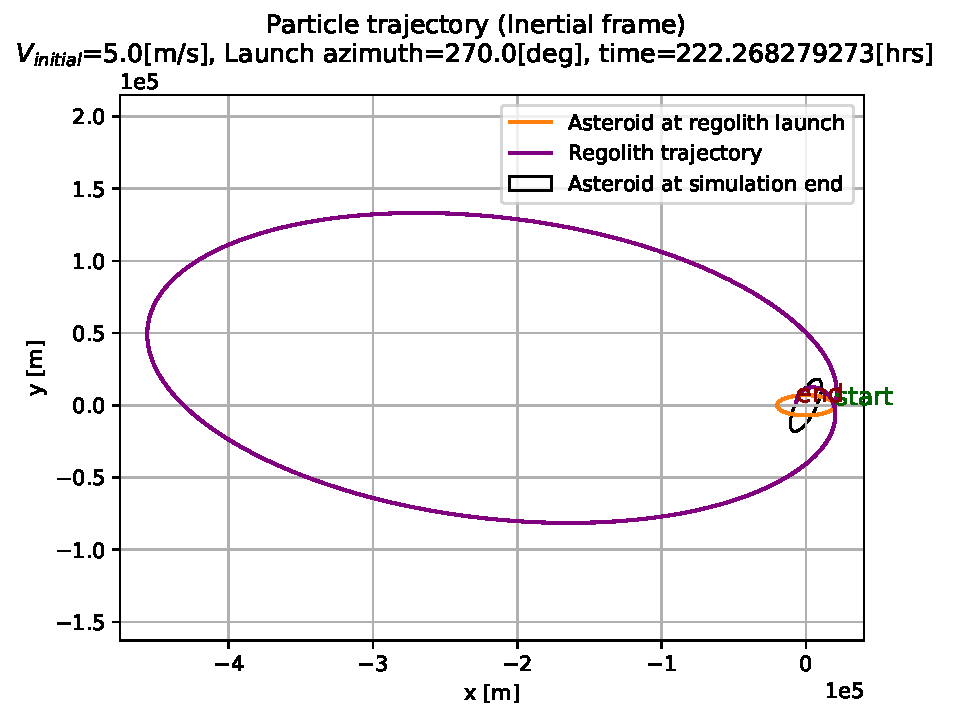
\includegraphics[width=0.5\textwidth, height=0.5\textheight, keepaspectratio=true]{Images/longest_edge_no_perturbations/5ms_270Azim_reimpact.pdf}
    \label{fig:5ms_270Azim_traj_noSP}
}
\caption{Regolith trajectory, expressed in the \gls{AIF}, for particles launched with azimuth \SI{270}{\degree} and velocity of \protect\subref{fig:4ms_270Azim_traj_noSP} \SI{4}{\metre\per\second} and \protect\subref{fig:5ms_270Azim_traj_noSP} \SI{5}{\metre\per\second}.}
\label{fig:270Azim_traj_noSP}
\end{figure}
\FloatBarrier
%%%
%%%
\begin{figure}[htb]
\centering
\captionsetup{justification=centering}
\subfloat[]{
    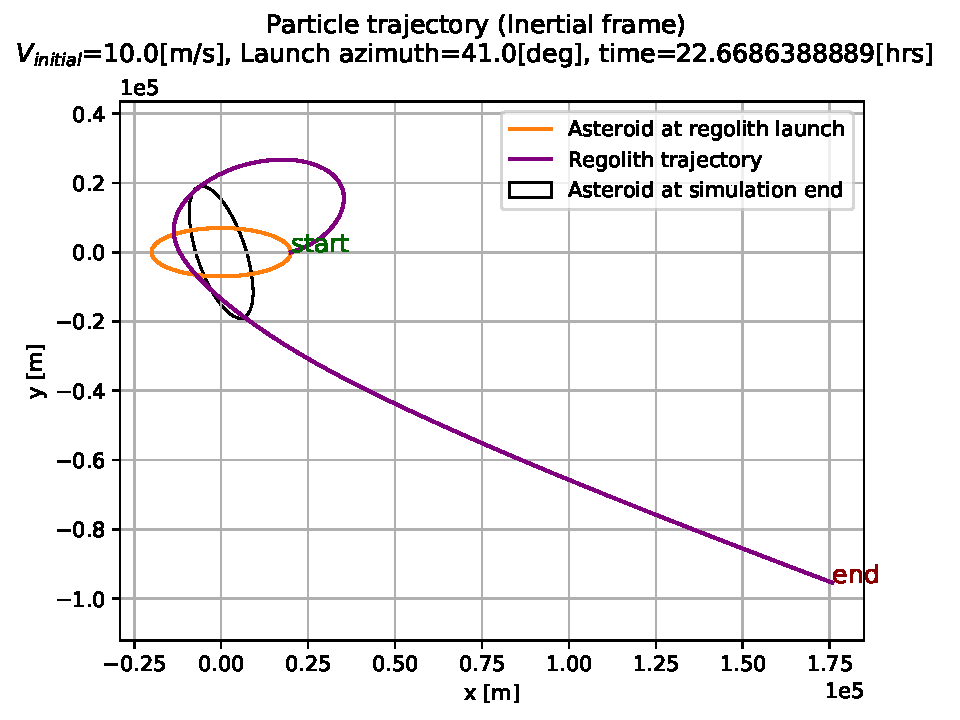
\includegraphics[width=0.5\textwidth, height=0.5\textheight, keepaspectratio=true]{Images/longest_edge_no_perturbations/10ms_41Azim_escape.pdf}
    \label{fig:10ms_41Azim_traj_noSP}
}
\subfloat[]{
    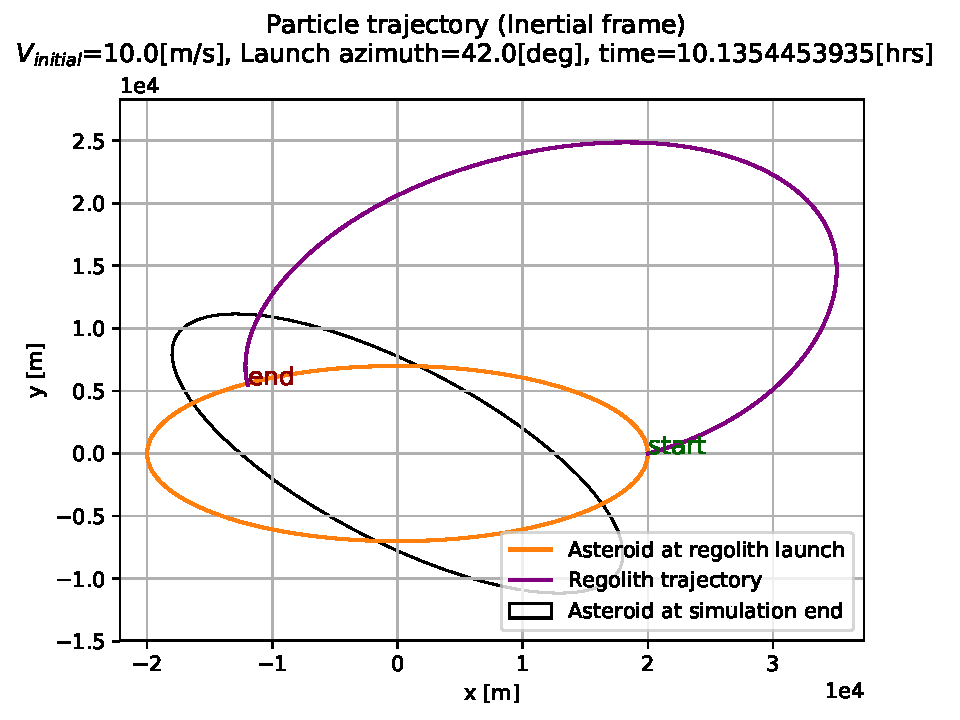
\includegraphics[width=0.5\textwidth, height=0.5\textheight, keepaspectratio=true]{Images/longest_edge_no_perturbations/10ms_42Azim_reimpact.pdf}
    \label{fig:10ms_42Azim_traj_noSP}
}
\caption{Regolith trajectory, expressed in the \gls{AIF}, for particles launched with velocity \SI{10}{\metre\per\second} and azimuth of \protect\subref{fig:10ms_41Azim_traj_noSP} \SI{41}{\degree} and \protect\subref{fig:10ms_42Azim_traj_noSP} \SI{42}{\degree}.}
\label{fig:10ms_traj_noSP}
\end{figure}
\FloatBarrier
%%%
